% =============================================================================
% 05-addressing-cpu-bus-notes.tex — Lecture Notes for Week 5:
% Addressing Modes, CPU Organization, and Bus Structures
%
% DERIVED ARTIFACT. Source of truth: Slides/CS401/05-addressing-cpu-bus.tex.
% Generated by /lecture-notes; do not hand-edit content independently of the
% Beamer source without re-running /qa-notes afterward (single-source-of-truth.md).
% Structured as a textbook chapter (numbered sections/figures/examples,
% topic-organized rather than a frame-by-frame transcript) per the project's
% textbook-chapter convention for Notes.
%
% Anchor reading: Hamacher, Computer Organization, 5th ed., Ch. 7 (addressing
%                 modes, bus organization) — cited at chapter level only; this
%                 course's Hamacher2002 index does not exist yet (the supplied
%                 PDF has no text layer and this environment lacks a page-
%                 rasterization tool for OCR — see knowledge-base-CS401.md's
%                 Anchor Textbooks table).
%                 Mano, Computer System Architecture, 3rd ed., Ch. 8 (Central
%                 Processing Unit: common bus system, stack organization,
%                 addressing modes) — page-cited from
%                 master_supporting_docs/CS401/supporting_books/Mano1993/index.md,
%                 built and verified 2026-08-06. (This corrects a prior
%                 mis-citation of Mano Ch. 7, which is actually Microprogrammed
%                 Control — Weeks 6-7's material, not this lecture's.)
%
% Compile with: cd Notes/CS401 &&
%   TEXINPUTS=../../Preambles:$TEXINPUTS xelatex -interaction=nonstopmode 05-addressing-cpu-bus-notes.tex
%   BIBINPUTS=../..:$BIBINPUTS bibtex 05-addressing-cpu-bus-notes
%   TEXINPUTS=../../Preambles:$TEXINPUTS xelatex -interaction=nonstopmode 05-addressing-cpu-bus-notes.tex  (x2)
%   (Windows/MiKTeX: use ; not : as the TEXINPUTS/BIBINPUTS separator)
% =============================================================================

\documentclass[11pt]{article}
\usepackage[margin=1in]{geometry}
% =============================================================================
% Preambles/header.tex — shared LaTeX/Beamer preamble for this project
%
% Use from a Beamer lecture by prepending:
%     % =============================================================================
% Preambles/header.tex — shared LaTeX/Beamer preamble for this project
%
% Use from a Beamer lecture by prepending:
%     % =============================================================================
% Preambles/header.tex — shared LaTeX/Beamer preamble for this project
%
% Use from a Beamer lecture by prepending:
%     \input{header}
% and compiling with TEXINPUTS=../Preambles:$TEXINPUTS (the /compile-latex
% skill does this automatically).
%
% PALETTE CONTRACT. Color names defined here MUST match the names in
% Quarto/theme-template.scss so Beamer and Quarto renderings use the same
% palette. The scripts/check-palette-sync.sh script enforces this.
%
% To customize: edit the HEX values below AND the matching $variable in
% Quarto/theme-template.scss, then run scripts/check-palette-sync.sh.
%
% TITLE PAGE. A formal, serif (Libertine) title-page template is defined in
% the Beamer-only block below (\setbeamertemplate{title page}) -- title,
% subtitle, a thin gold rule, then \author/\institute/\date. Frametitle and
% body text remain on Beamer's sans-serif default. No SCSS counterpart is
% needed for this (font/layout only, no new colors).
% =============================================================================

% -----------------------------------------------------------------------------
% Engine detection + encoding
%
% Our /compile-latex skill uses XeLaTeX, where inputenc is unnecessary and
% can produce encoding warnings. Only load inputenc under pdfTeX.
% -----------------------------------------------------------------------------
\usepackage{iftex}
\ifPDFTeX
  \usepackage[utf8]{inputenc}
\fi

\usepackage{amsmath, amssymb, amsthm}
\usepackage{booktabs}
\usepackage{graphicx}

% -----------------------------------------------------------------------------
% Serif face for the title page (formal/academic look). Linux Libertine is
% XeLaTeX- and pdfTeX-safe and redefines \rmdefault, so \rmfamily picks it up
% everywhere \rmfamily is used explicitly. Body text and frametitles stay on
% Beamer's own sans-serif default (unaffected) -- only the title-page
% \setbeamerfont{...} overrides below opt in to \rmfamily.
% -----------------------------------------------------------------------------
\usepackage{libertine}

% -----------------------------------------------------------------------------
% PALETTE — mirrors Quarto/theme-template.scss variable names.
% Load xcolor and define colors BEFORE anything that references them
% (notably hyperref, hypersetup, and the Beamer color assignments).
% -----------------------------------------------------------------------------
\usepackage{xcolor}

\definecolor{primary-blue}{HTML}{012169}      % headings, accents
\definecolor{primary-gold}{HTML}{B9975B}      % emphasis, borders
\definecolor{highlight-yellow}{HTML}{F2A900}  % markers, alerts
\definecolor{light-bg}{HTML}{E8EDF5}          % title / section backgrounds
\definecolor{jet}{HTML}{1A1A1A}               % body text

% Semantic colors (used in diagrams and annotations)
\definecolor{positive}{HTML}{15803D}          % good / observed / identified
\definecolor{negative}{HTML}{B91C1C}          % bad / problematic / bias
\definecolor{neutral}{HTML}{525252}           % reference / context

% Highlight accents (match .hi-* classes in the SCSS)
\definecolor{hi-slate}{HTML}{314F4F}
\definecolor{hi-green}{HTML}{2E8B57}
\definecolor{hi-red}{HTML}{C41E3A}

% Semantic aliases so skill templates and snippets can write
% \textcolor{accent}{...} without hard-coding "primary-blue".
\colorlet{accent}{primary-blue}
\colorlet{accent2}{primary-gold}

% -----------------------------------------------------------------------------
% Hyperref — loaded AFTER xcolor + palette so link colors resolve.
% -----------------------------------------------------------------------------
\usepackage{hyperref}
\hypersetup{colorlinks=true, linkcolor=primary-blue, urlcolor=primary-blue,
            citecolor=primary-blue, pdfborder={0 0 0}}

% -----------------------------------------------------------------------------
% Course code — set once per deck (after \input{header}, before \begin{document})
% via \coursecode{CS401}. Shown in the footer on every slide so a deck's course
% is identifiable without opening the title page. Empty by default.
% -----------------------------------------------------------------------------
\makeatletter
\newcommand{\coursecode}[1]{\gdef\@coursecodetext{#1}}
\gdef\@coursecodetext{}
\makeatother

% -----------------------------------------------------------------------------
% Beamer theme assignments (only apply under Beamer).
%
% We detect Beamer via \@ifclassloaded{beamer}, which is the documented,
% non-internal way. This must be wrapped in \makeatletter/\makeatother
% because \@ifclassloaded contains an @-catcode character.
% -----------------------------------------------------------------------------
\makeatletter
\@ifclassloaded{beamer}{%
  \usefonttheme{professionalfonts}
  \setbeamercolor{structure}{fg=primary-blue}
  \setbeamercolor{frametitle}{fg=primary-blue}
  \setbeamercolor{title}{fg=primary-blue}
  \setbeamercolor{subtitle}{fg=primary-gold}
  \setbeamercolor{author}{fg=primary-blue}
  \setbeamercolor{institute}{fg=neutral}
  \setbeamercolor{date}{fg=primary-gold}
  \setbeamercolor{itemize item}{fg=primary-blue}
  \setbeamercolor{itemize subitem}{fg=primary-gold}
  \setbeamercolor{alerted text}{fg=primary-gold}
  \setbeamercolor{block title}{fg=white, bg=primary-blue}
  \setbeamercolor{block body}{bg=light-bg}
  % Semantic block variants: block=definition/concept (blue), exampleblock=
  % worked example (green/positive), alertblock=key takeaway or caution (gold).
  % Keep to <=2 colored boxes per slide across ALL three variants (INV-7).
  \setbeamercolor{block title example}{fg=white, bg=positive}
  \setbeamercolor{block body example}{bg=light-bg}
  \setbeamercolor{block title alerted}{fg=white, bg=primary-gold}
  \setbeamercolor{block body alerted}{bg=light-bg}

  % ---------------------------------------------------------------------------
  % Formal title page: serif (Libertine, via \rmfamily) for title-page
  % elements only. Body text, itemize, and frametitle are intentionally left
  % on Beamer's sans-serif default -- \usebeamerfont{title} is also what
  % \transitionslide (below) uses for its big centered text, so section
  % transitions pick up the same serif treatment for free.
  % ---------------------------------------------------------------------------
  \setbeamerfont{title}{family=\rmfamily, series=\bfseries, size=\Large}
  \setbeamerfont{subtitle}{family=\rmfamily, shape=\itshape, size=\normalsize}
  \setbeamerfont{author}{family=\rmfamily, size=\normalsize}
  \setbeamerfont{institute}{family=\rmfamily, size=\scriptsize}
  \setbeamerfont{date}{family=\rmfamily, size=\scriptsize}

  \setbeamertemplate{title page}{
    \vfill
    \begin{center}
      {\usebeamerfont{title}\usebeamercolor[fg]{title}\inserttitle\par}
      \vspace{0.15cm}
      {\usebeamerfont{subtitle}\usebeamercolor[fg]{subtitle}\insertsubtitle\par}
      \vspace{0.45cm}
      {\color{primary-gold}\rule{0.42\textwidth}{0.6pt}\par}
      \vspace{0.45cm}
      {\usebeamerfont{author}\usebeamercolor[fg]{author}\insertauthor\par}
      \vspace{0.35cm}
      {\usebeamerfont{institute}\usebeamercolor[fg]{institute}\insertinstitute\par}
      \vspace{0.35cm}
      {\usebeamerfont{date}\usebeamercolor[fg]{date}\insertdate\par}
    \end{center}
    \vfill
  }

  % Minimal footer: course code (left) + page X / N (right), no navigation clutter
  \setbeamertemplate{navigation symbols}{}
  \setbeamertemplate{footline}{%
    \color{neutral}\footnotesize\hspace{0.7em}\@coursecodetext\hfill
    \insertframenumber/\inserttotalframenumber\hspace{0.7em}\vspace{0.3em}}
}{}
\makeatother

% -----------------------------------------------------------------------------
% TikZ setup — libraries the snippet gallery uses
% -----------------------------------------------------------------------------
\usepackage{tikz}
\usetikzlibrary{arrows.meta, positioning, calc, decorations.pathreplacing,
                fit, shapes.geometric, backgrounds}

% Shared TikZ styles — snippets and hand-written diagrams can pick these up
% via `\begin{tikzpicture}[every node/.style={...}]` or by naming specific
% styles (e.g., `\node[dag-node] (X) at (0,0) {X};`).
\tikzset{
  % Node styles for causal DAGs and similar
  dag-node/.style = {
    draw=primary-blue, fill=light-bg, rounded corners=2pt,
    minimum width=1.2cm, minimum height=0.9cm, align=center, font=\small
  },
  decision-node/.style = {
    draw=primary-gold, fill=white, diamond, aspect=1.8,
    minimum width=1.8cm, minimum height=1.2cm, align=center, font=\small,
    inner sep=1pt
  },
  % Edge styles — observed vs counterfactual
  observed-edge/.style = {-{Latex[length=2.5mm]}, thick, draw=jet},
  counterfactual-edge/.style = {-{Latex[length=2.5mm]}, thick, draw=neutral, dashed},
  confound-edge/.style = {-{Latex[length=2.5mm]}, thick, draw=negative, dashed},
  % Data-point styles for plots
  observed-dot/.style = {fill=primary-blue, draw=primary-blue, circle, inner sep=1.2pt},
  counterfactual-dot/.style = {fill=white, draw=neutral, circle, inner sep=1.2pt}
}

% -----------------------------------------------------------------------------
% Convenience macros
% -----------------------------------------------------------------------------
\newcommand{\muted}[1]{\textcolor{neutral}{#1}}
\newcommand{\key}[1]{\textcolor{primary-gold}{\textbf{#1}}}
\newcommand{\good}[1]{\textcolor{positive}{#1}}
\newcommand{\bad}[1]{\textcolor{negative}{#1}}

% Standout frame macro: full-bleed dark background for section transitions.
% Beamer-only (uses \begin{frame}/\setbeamercolor/\usebeamerfont) -- do not
% call from an article-class file (e.g. Notes/<CODE>/*-notes.tex). \muted,
% \key, \good, \bad, and \coursecode above are plain xcolor/gdef and are
% safe to use from either class; verified when Notes/article-class support
% was added.
% Expand: \transitionslide{Your transition title}
\newcommand{\transitionslide}[1]{%
  \begingroup
  \setbeamercolor{background canvas}{bg=primary-blue}
  \begin{frame}[plain]
    \centering
    \vfill
    {\usebeamerfont{title}\color{white}\Large #1\par}
    \vfill
  \end{frame}
  \endgroup
}

% and compiling with TEXINPUTS=../Preambles:$TEXINPUTS (the /compile-latex
% skill does this automatically).
%
% PALETTE CONTRACT. Color names defined here MUST match the names in
% Quarto/theme-template.scss so Beamer and Quarto renderings use the same
% palette. The scripts/check-palette-sync.sh script enforces this.
%
% To customize: edit the HEX values below AND the matching $variable in
% Quarto/theme-template.scss, then run scripts/check-palette-sync.sh.
%
% TITLE PAGE. A formal, serif (Libertine) title-page template is defined in
% the Beamer-only block below (\setbeamertemplate{title page}) -- title,
% subtitle, a thin gold rule, then \author/\institute/\date. Frametitle and
% body text remain on Beamer's sans-serif default. No SCSS counterpart is
% needed for this (font/layout only, no new colors).
% =============================================================================

% -----------------------------------------------------------------------------
% Engine detection + encoding
%
% Our /compile-latex skill uses XeLaTeX, where inputenc is unnecessary and
% can produce encoding warnings. Only load inputenc under pdfTeX.
% -----------------------------------------------------------------------------
\usepackage{iftex}
\ifPDFTeX
  \usepackage[utf8]{inputenc}
\fi

\usepackage{amsmath, amssymb, amsthm}
\usepackage{booktabs}
\usepackage{graphicx}

% -----------------------------------------------------------------------------
% Serif face for the title page (formal/academic look). Linux Libertine is
% XeLaTeX- and pdfTeX-safe and redefines \rmdefault, so \rmfamily picks it up
% everywhere \rmfamily is used explicitly. Body text and frametitles stay on
% Beamer's own sans-serif default (unaffected) -- only the title-page
% \setbeamerfont{...} overrides below opt in to \rmfamily.
% -----------------------------------------------------------------------------
\usepackage{libertine}

% -----------------------------------------------------------------------------
% PALETTE — mirrors Quarto/theme-template.scss variable names.
% Load xcolor and define colors BEFORE anything that references them
% (notably hyperref, hypersetup, and the Beamer color assignments).
% -----------------------------------------------------------------------------
\usepackage{xcolor}

\definecolor{primary-blue}{HTML}{012169}      % headings, accents
\definecolor{primary-gold}{HTML}{B9975B}      % emphasis, borders
\definecolor{highlight-yellow}{HTML}{F2A900}  % markers, alerts
\definecolor{light-bg}{HTML}{E8EDF5}          % title / section backgrounds
\definecolor{jet}{HTML}{1A1A1A}               % body text

% Semantic colors (used in diagrams and annotations)
\definecolor{positive}{HTML}{15803D}          % good / observed / identified
\definecolor{negative}{HTML}{B91C1C}          % bad / problematic / bias
\definecolor{neutral}{HTML}{525252}           % reference / context

% Highlight accents (match .hi-* classes in the SCSS)
\definecolor{hi-slate}{HTML}{314F4F}
\definecolor{hi-green}{HTML}{2E8B57}
\definecolor{hi-red}{HTML}{C41E3A}

% Semantic aliases so skill templates and snippets can write
% \textcolor{accent}{...} without hard-coding "primary-blue".
\colorlet{accent}{primary-blue}
\colorlet{accent2}{primary-gold}

% -----------------------------------------------------------------------------
% Hyperref — loaded AFTER xcolor + palette so link colors resolve.
% -----------------------------------------------------------------------------
\usepackage{hyperref}
\hypersetup{colorlinks=true, linkcolor=primary-blue, urlcolor=primary-blue,
            citecolor=primary-blue, pdfborder={0 0 0}}

% -----------------------------------------------------------------------------
% Course code — set once per deck (after % =============================================================================
% Preambles/header.tex — shared LaTeX/Beamer preamble for this project
%
% Use from a Beamer lecture by prepending:
%     \input{header}
% and compiling with TEXINPUTS=../Preambles:$TEXINPUTS (the /compile-latex
% skill does this automatically).
%
% PALETTE CONTRACT. Color names defined here MUST match the names in
% Quarto/theme-template.scss so Beamer and Quarto renderings use the same
% palette. The scripts/check-palette-sync.sh script enforces this.
%
% To customize: edit the HEX values below AND the matching $variable in
% Quarto/theme-template.scss, then run scripts/check-palette-sync.sh.
%
% TITLE PAGE. A formal, serif (Libertine) title-page template is defined in
% the Beamer-only block below (\setbeamertemplate{title page}) -- title,
% subtitle, a thin gold rule, then \author/\institute/\date. Frametitle and
% body text remain on Beamer's sans-serif default. No SCSS counterpart is
% needed for this (font/layout only, no new colors).
% =============================================================================

% -----------------------------------------------------------------------------
% Engine detection + encoding
%
% Our /compile-latex skill uses XeLaTeX, where inputenc is unnecessary and
% can produce encoding warnings. Only load inputenc under pdfTeX.
% -----------------------------------------------------------------------------
\usepackage{iftex}
\ifPDFTeX
  \usepackage[utf8]{inputenc}
\fi

\usepackage{amsmath, amssymb, amsthm}
\usepackage{booktabs}
\usepackage{graphicx}

% -----------------------------------------------------------------------------
% Serif face for the title page (formal/academic look). Linux Libertine is
% XeLaTeX- and pdfTeX-safe and redefines \rmdefault, so \rmfamily picks it up
% everywhere \rmfamily is used explicitly. Body text and frametitles stay on
% Beamer's own sans-serif default (unaffected) -- only the title-page
% \setbeamerfont{...} overrides below opt in to \rmfamily.
% -----------------------------------------------------------------------------
\usepackage{libertine}

% -----------------------------------------------------------------------------
% PALETTE — mirrors Quarto/theme-template.scss variable names.
% Load xcolor and define colors BEFORE anything that references them
% (notably hyperref, hypersetup, and the Beamer color assignments).
% -----------------------------------------------------------------------------
\usepackage{xcolor}

\definecolor{primary-blue}{HTML}{012169}      % headings, accents
\definecolor{primary-gold}{HTML}{B9975B}      % emphasis, borders
\definecolor{highlight-yellow}{HTML}{F2A900}  % markers, alerts
\definecolor{light-bg}{HTML}{E8EDF5}          % title / section backgrounds
\definecolor{jet}{HTML}{1A1A1A}               % body text

% Semantic colors (used in diagrams and annotations)
\definecolor{positive}{HTML}{15803D}          % good / observed / identified
\definecolor{negative}{HTML}{B91C1C}          % bad / problematic / bias
\definecolor{neutral}{HTML}{525252}           % reference / context

% Highlight accents (match .hi-* classes in the SCSS)
\definecolor{hi-slate}{HTML}{314F4F}
\definecolor{hi-green}{HTML}{2E8B57}
\definecolor{hi-red}{HTML}{C41E3A}

% Semantic aliases so skill templates and snippets can write
% \textcolor{accent}{...} without hard-coding "primary-blue".
\colorlet{accent}{primary-blue}
\colorlet{accent2}{primary-gold}

% -----------------------------------------------------------------------------
% Hyperref — loaded AFTER xcolor + palette so link colors resolve.
% -----------------------------------------------------------------------------
\usepackage{hyperref}
\hypersetup{colorlinks=true, linkcolor=primary-blue, urlcolor=primary-blue,
            citecolor=primary-blue, pdfborder={0 0 0}}

% -----------------------------------------------------------------------------
% Course code — set once per deck (after \input{header}, before \begin{document})
% via \coursecode{CS401}. Shown in the footer on every slide so a deck's course
% is identifiable without opening the title page. Empty by default.
% -----------------------------------------------------------------------------
\makeatletter
\newcommand{\coursecode}[1]{\gdef\@coursecodetext{#1}}
\gdef\@coursecodetext{}
\makeatother

% -----------------------------------------------------------------------------
% Beamer theme assignments (only apply under Beamer).
%
% We detect Beamer via \@ifclassloaded{beamer}, which is the documented,
% non-internal way. This must be wrapped in \makeatletter/\makeatother
% because \@ifclassloaded contains an @-catcode character.
% -----------------------------------------------------------------------------
\makeatletter
\@ifclassloaded{beamer}{%
  \usefonttheme{professionalfonts}
  \setbeamercolor{structure}{fg=primary-blue}
  \setbeamercolor{frametitle}{fg=primary-blue}
  \setbeamercolor{title}{fg=primary-blue}
  \setbeamercolor{subtitle}{fg=primary-gold}
  \setbeamercolor{author}{fg=primary-blue}
  \setbeamercolor{institute}{fg=neutral}
  \setbeamercolor{date}{fg=primary-gold}
  \setbeamercolor{itemize item}{fg=primary-blue}
  \setbeamercolor{itemize subitem}{fg=primary-gold}
  \setbeamercolor{alerted text}{fg=primary-gold}
  \setbeamercolor{block title}{fg=white, bg=primary-blue}
  \setbeamercolor{block body}{bg=light-bg}
  % Semantic block variants: block=definition/concept (blue), exampleblock=
  % worked example (green/positive), alertblock=key takeaway or caution (gold).
  % Keep to <=2 colored boxes per slide across ALL three variants (INV-7).
  \setbeamercolor{block title example}{fg=white, bg=positive}
  \setbeamercolor{block body example}{bg=light-bg}
  \setbeamercolor{block title alerted}{fg=white, bg=primary-gold}
  \setbeamercolor{block body alerted}{bg=light-bg}

  % ---------------------------------------------------------------------------
  % Formal title page: serif (Libertine, via \rmfamily) for title-page
  % elements only. Body text, itemize, and frametitle are intentionally left
  % on Beamer's sans-serif default -- \usebeamerfont{title} is also what
  % \transitionslide (below) uses for its big centered text, so section
  % transitions pick up the same serif treatment for free.
  % ---------------------------------------------------------------------------
  \setbeamerfont{title}{family=\rmfamily, series=\bfseries, size=\Large}
  \setbeamerfont{subtitle}{family=\rmfamily, shape=\itshape, size=\normalsize}
  \setbeamerfont{author}{family=\rmfamily, size=\normalsize}
  \setbeamerfont{institute}{family=\rmfamily, size=\scriptsize}
  \setbeamerfont{date}{family=\rmfamily, size=\scriptsize}

  \setbeamertemplate{title page}{
    \vfill
    \begin{center}
      {\usebeamerfont{title}\usebeamercolor[fg]{title}\inserttitle\par}
      \vspace{0.15cm}
      {\usebeamerfont{subtitle}\usebeamercolor[fg]{subtitle}\insertsubtitle\par}
      \vspace{0.45cm}
      {\color{primary-gold}\rule{0.42\textwidth}{0.6pt}\par}
      \vspace{0.45cm}
      {\usebeamerfont{author}\usebeamercolor[fg]{author}\insertauthor\par}
      \vspace{0.35cm}
      {\usebeamerfont{institute}\usebeamercolor[fg]{institute}\insertinstitute\par}
      \vspace{0.35cm}
      {\usebeamerfont{date}\usebeamercolor[fg]{date}\insertdate\par}
    \end{center}
    \vfill
  }

  % Minimal footer: course code (left) + page X / N (right), no navigation clutter
  \setbeamertemplate{navigation symbols}{}
  \setbeamertemplate{footline}{%
    \color{neutral}\footnotesize\hspace{0.7em}\@coursecodetext\hfill
    \insertframenumber/\inserttotalframenumber\hspace{0.7em}\vspace{0.3em}}
}{}
\makeatother

% -----------------------------------------------------------------------------
% TikZ setup — libraries the snippet gallery uses
% -----------------------------------------------------------------------------
\usepackage{tikz}
\usetikzlibrary{arrows.meta, positioning, calc, decorations.pathreplacing,
                fit, shapes.geometric, backgrounds}

% Shared TikZ styles — snippets and hand-written diagrams can pick these up
% via `\begin{tikzpicture}[every node/.style={...}]` or by naming specific
% styles (e.g., `\node[dag-node] (X) at (0,0) {X};`).
\tikzset{
  % Node styles for causal DAGs and similar
  dag-node/.style = {
    draw=primary-blue, fill=light-bg, rounded corners=2pt,
    minimum width=1.2cm, minimum height=0.9cm, align=center, font=\small
  },
  decision-node/.style = {
    draw=primary-gold, fill=white, diamond, aspect=1.8,
    minimum width=1.8cm, minimum height=1.2cm, align=center, font=\small,
    inner sep=1pt
  },
  % Edge styles — observed vs counterfactual
  observed-edge/.style = {-{Latex[length=2.5mm]}, thick, draw=jet},
  counterfactual-edge/.style = {-{Latex[length=2.5mm]}, thick, draw=neutral, dashed},
  confound-edge/.style = {-{Latex[length=2.5mm]}, thick, draw=negative, dashed},
  % Data-point styles for plots
  observed-dot/.style = {fill=primary-blue, draw=primary-blue, circle, inner sep=1.2pt},
  counterfactual-dot/.style = {fill=white, draw=neutral, circle, inner sep=1.2pt}
}

% -----------------------------------------------------------------------------
% Convenience macros
% -----------------------------------------------------------------------------
\newcommand{\muted}[1]{\textcolor{neutral}{#1}}
\newcommand{\key}[1]{\textcolor{primary-gold}{\textbf{#1}}}
\newcommand{\good}[1]{\textcolor{positive}{#1}}
\newcommand{\bad}[1]{\textcolor{negative}{#1}}

% Standout frame macro: full-bleed dark background for section transitions.
% Beamer-only (uses \begin{frame}/\setbeamercolor/\usebeamerfont) -- do not
% call from an article-class file (e.g. Notes/<CODE>/*-notes.tex). \muted,
% \key, \good, \bad, and \coursecode above are plain xcolor/gdef and are
% safe to use from either class; verified when Notes/article-class support
% was added.
% Expand: \transitionslide{Your transition title}
\newcommand{\transitionslide}[1]{%
  \begingroup
  \setbeamercolor{background canvas}{bg=primary-blue}
  \begin{frame}[plain]
    \centering
    \vfill
    {\usebeamerfont{title}\color{white}\Large #1\par}
    \vfill
  \end{frame}
  \endgroup
}
, before \begin{document})
% via \coursecode{CS401}. Shown in the footer on every slide so a deck's course
% is identifiable without opening the title page. Empty by default.
% -----------------------------------------------------------------------------
\makeatletter
\newcommand{\coursecode}[1]{\gdef\@coursecodetext{#1}}
\gdef\@coursecodetext{}
\makeatother

% -----------------------------------------------------------------------------
% Beamer theme assignments (only apply under Beamer).
%
% We detect Beamer via \@ifclassloaded{beamer}, which is the documented,
% non-internal way. This must be wrapped in \makeatletter/\makeatother
% because \@ifclassloaded contains an @-catcode character.
% -----------------------------------------------------------------------------
\makeatletter
\@ifclassloaded{beamer}{%
  \usefonttheme{professionalfonts}
  \setbeamercolor{structure}{fg=primary-blue}
  \setbeamercolor{frametitle}{fg=primary-blue}
  \setbeamercolor{title}{fg=primary-blue}
  \setbeamercolor{subtitle}{fg=primary-gold}
  \setbeamercolor{author}{fg=primary-blue}
  \setbeamercolor{institute}{fg=neutral}
  \setbeamercolor{date}{fg=primary-gold}
  \setbeamercolor{itemize item}{fg=primary-blue}
  \setbeamercolor{itemize subitem}{fg=primary-gold}
  \setbeamercolor{alerted text}{fg=primary-gold}
  \setbeamercolor{block title}{fg=white, bg=primary-blue}
  \setbeamercolor{block body}{bg=light-bg}
  % Semantic block variants: block=definition/concept (blue), exampleblock=
  % worked example (green/positive), alertblock=key takeaway or caution (gold).
  % Keep to <=2 colored boxes per slide across ALL three variants (INV-7).
  \setbeamercolor{block title example}{fg=white, bg=positive}
  \setbeamercolor{block body example}{bg=light-bg}
  \setbeamercolor{block title alerted}{fg=white, bg=primary-gold}
  \setbeamercolor{block body alerted}{bg=light-bg}

  % ---------------------------------------------------------------------------
  % Formal title page: serif (Libertine, via \rmfamily) for title-page
  % elements only. Body text, itemize, and frametitle are intentionally left
  % on Beamer's sans-serif default -- \usebeamerfont{title} is also what
  % \transitionslide (below) uses for its big centered text, so section
  % transitions pick up the same serif treatment for free.
  % ---------------------------------------------------------------------------
  \setbeamerfont{title}{family=\rmfamily, series=\bfseries, size=\Large}
  \setbeamerfont{subtitle}{family=\rmfamily, shape=\itshape, size=\normalsize}
  \setbeamerfont{author}{family=\rmfamily, size=\normalsize}
  \setbeamerfont{institute}{family=\rmfamily, size=\scriptsize}
  \setbeamerfont{date}{family=\rmfamily, size=\scriptsize}

  \setbeamertemplate{title page}{
    \vfill
    \begin{center}
      {\usebeamerfont{title}\usebeamercolor[fg]{title}\inserttitle\par}
      \vspace{0.15cm}
      {\usebeamerfont{subtitle}\usebeamercolor[fg]{subtitle}\insertsubtitle\par}
      \vspace{0.45cm}
      {\color{primary-gold}\rule{0.42\textwidth}{0.6pt}\par}
      \vspace{0.45cm}
      {\usebeamerfont{author}\usebeamercolor[fg]{author}\insertauthor\par}
      \vspace{0.35cm}
      {\usebeamerfont{institute}\usebeamercolor[fg]{institute}\insertinstitute\par}
      \vspace{0.35cm}
      {\usebeamerfont{date}\usebeamercolor[fg]{date}\insertdate\par}
    \end{center}
    \vfill
  }

  % Minimal footer: course code (left) + page X / N (right), no navigation clutter
  \setbeamertemplate{navigation symbols}{}
  \setbeamertemplate{footline}{%
    \color{neutral}\footnotesize\hspace{0.7em}\@coursecodetext\hfill
    \insertframenumber/\inserttotalframenumber\hspace{0.7em}\vspace{0.3em}}
}{}
\makeatother

% -----------------------------------------------------------------------------
% TikZ setup — libraries the snippet gallery uses
% -----------------------------------------------------------------------------
\usepackage{tikz}
\usetikzlibrary{arrows.meta, positioning, calc, decorations.pathreplacing,
                fit, shapes.geometric, backgrounds}

% Shared TikZ styles — snippets and hand-written diagrams can pick these up
% via `\begin{tikzpicture}[every node/.style={...}]` or by naming specific
% styles (e.g., `\node[dag-node] (X) at (0,0) {X};`).
\tikzset{
  % Node styles for causal DAGs and similar
  dag-node/.style = {
    draw=primary-blue, fill=light-bg, rounded corners=2pt,
    minimum width=1.2cm, minimum height=0.9cm, align=center, font=\small
  },
  decision-node/.style = {
    draw=primary-gold, fill=white, diamond, aspect=1.8,
    minimum width=1.8cm, minimum height=1.2cm, align=center, font=\small,
    inner sep=1pt
  },
  % Edge styles — observed vs counterfactual
  observed-edge/.style = {-{Latex[length=2.5mm]}, thick, draw=jet},
  counterfactual-edge/.style = {-{Latex[length=2.5mm]}, thick, draw=neutral, dashed},
  confound-edge/.style = {-{Latex[length=2.5mm]}, thick, draw=negative, dashed},
  % Data-point styles for plots
  observed-dot/.style = {fill=primary-blue, draw=primary-blue, circle, inner sep=1.2pt},
  counterfactual-dot/.style = {fill=white, draw=neutral, circle, inner sep=1.2pt}
}

% -----------------------------------------------------------------------------
% Convenience macros
% -----------------------------------------------------------------------------
\newcommand{\muted}[1]{\textcolor{neutral}{#1}}
\newcommand{\key}[1]{\textcolor{primary-gold}{\textbf{#1}}}
\newcommand{\good}[1]{\textcolor{positive}{#1}}
\newcommand{\bad}[1]{\textcolor{negative}{#1}}

% Standout frame macro: full-bleed dark background for section transitions.
% Beamer-only (uses \begin{frame}/\setbeamercolor/\usebeamerfont) -- do not
% call from an article-class file (e.g. Notes/<CODE>/*-notes.tex). \muted,
% \key, \good, \bad, and \coursecode above are plain xcolor/gdef and are
% safe to use from either class; verified when Notes/article-class support
% was added.
% Expand: \transitionslide{Your transition title}
\newcommand{\transitionslide}[1]{%
  \begingroup
  \setbeamercolor{background canvas}{bg=primary-blue}
  \begin{frame}[plain]
    \centering
    \vfill
    {\usebeamerfont{title}\color{white}\Large #1\par}
    \vfill
  \end{frame}
  \endgroup
}

% and compiling with TEXINPUTS=../Preambles:$TEXINPUTS (the /compile-latex
% skill does this automatically).
%
% PALETTE CONTRACT. Color names defined here MUST match the names in
% Quarto/theme-template.scss so Beamer and Quarto renderings use the same
% palette. The scripts/check-palette-sync.sh script enforces this.
%
% To customize: edit the HEX values below AND the matching $variable in
% Quarto/theme-template.scss, then run scripts/check-palette-sync.sh.
%
% TITLE PAGE. A formal, serif (Libertine) title-page template is defined in
% the Beamer-only block below (\setbeamertemplate{title page}) -- title,
% subtitle, a thin gold rule, then \author/\institute/\date. Frametitle and
% body text remain on Beamer's sans-serif default. No SCSS counterpart is
% needed for this (font/layout only, no new colors).
% =============================================================================

% -----------------------------------------------------------------------------
% Engine detection + encoding
%
% Our /compile-latex skill uses XeLaTeX, where inputenc is unnecessary and
% can produce encoding warnings. Only load inputenc under pdfTeX.
% -----------------------------------------------------------------------------
\usepackage{iftex}
\ifPDFTeX
  \usepackage[utf8]{inputenc}
\fi

\usepackage{amsmath, amssymb, amsthm}
\usepackage{booktabs}
\usepackage{graphicx}

% -----------------------------------------------------------------------------
% Serif face for the title page (formal/academic look). Linux Libertine is
% XeLaTeX- and pdfTeX-safe and redefines \rmdefault, so \rmfamily picks it up
% everywhere \rmfamily is used explicitly. Body text and frametitles stay on
% Beamer's own sans-serif default (unaffected) -- only the title-page
% \setbeamerfont{...} overrides below opt in to \rmfamily.
% -----------------------------------------------------------------------------
\usepackage{libertine}

% -----------------------------------------------------------------------------
% PALETTE — mirrors Quarto/theme-template.scss variable names.
% Load xcolor and define colors BEFORE anything that references them
% (notably hyperref, hypersetup, and the Beamer color assignments).
% -----------------------------------------------------------------------------
\usepackage{xcolor}

\definecolor{primary-blue}{HTML}{012169}      % headings, accents
\definecolor{primary-gold}{HTML}{B9975B}      % emphasis, borders
\definecolor{highlight-yellow}{HTML}{F2A900}  % markers, alerts
\definecolor{light-bg}{HTML}{E8EDF5}          % title / section backgrounds
\definecolor{jet}{HTML}{1A1A1A}               % body text

% Semantic colors (used in diagrams and annotations)
\definecolor{positive}{HTML}{15803D}          % good / observed / identified
\definecolor{negative}{HTML}{B91C1C}          % bad / problematic / bias
\definecolor{neutral}{HTML}{525252}           % reference / context

% Highlight accents (match .hi-* classes in the SCSS)
\definecolor{hi-slate}{HTML}{314F4F}
\definecolor{hi-green}{HTML}{2E8B57}
\definecolor{hi-red}{HTML}{C41E3A}

% Semantic aliases so skill templates and snippets can write
% \textcolor{accent}{...} without hard-coding "primary-blue".
\colorlet{accent}{primary-blue}
\colorlet{accent2}{primary-gold}

% -----------------------------------------------------------------------------
% Hyperref — loaded AFTER xcolor + palette so link colors resolve.
% -----------------------------------------------------------------------------
\usepackage{hyperref}
\hypersetup{colorlinks=true, linkcolor=primary-blue, urlcolor=primary-blue,
            citecolor=primary-blue, pdfborder={0 0 0}}

% -----------------------------------------------------------------------------
% Course code — set once per deck (after % =============================================================================
% Preambles/header.tex — shared LaTeX/Beamer preamble for this project
%
% Use from a Beamer lecture by prepending:
%     % =============================================================================
% Preambles/header.tex — shared LaTeX/Beamer preamble for this project
%
% Use from a Beamer lecture by prepending:
%     \input{header}
% and compiling with TEXINPUTS=../Preambles:$TEXINPUTS (the /compile-latex
% skill does this automatically).
%
% PALETTE CONTRACT. Color names defined here MUST match the names in
% Quarto/theme-template.scss so Beamer and Quarto renderings use the same
% palette. The scripts/check-palette-sync.sh script enforces this.
%
% To customize: edit the HEX values below AND the matching $variable in
% Quarto/theme-template.scss, then run scripts/check-palette-sync.sh.
%
% TITLE PAGE. A formal, serif (Libertine) title-page template is defined in
% the Beamer-only block below (\setbeamertemplate{title page}) -- title,
% subtitle, a thin gold rule, then \author/\institute/\date. Frametitle and
% body text remain on Beamer's sans-serif default. No SCSS counterpart is
% needed for this (font/layout only, no new colors).
% =============================================================================

% -----------------------------------------------------------------------------
% Engine detection + encoding
%
% Our /compile-latex skill uses XeLaTeX, where inputenc is unnecessary and
% can produce encoding warnings. Only load inputenc under pdfTeX.
% -----------------------------------------------------------------------------
\usepackage{iftex}
\ifPDFTeX
  \usepackage[utf8]{inputenc}
\fi

\usepackage{amsmath, amssymb, amsthm}
\usepackage{booktabs}
\usepackage{graphicx}

% -----------------------------------------------------------------------------
% Serif face for the title page (formal/academic look). Linux Libertine is
% XeLaTeX- and pdfTeX-safe and redefines \rmdefault, so \rmfamily picks it up
% everywhere \rmfamily is used explicitly. Body text and frametitles stay on
% Beamer's own sans-serif default (unaffected) -- only the title-page
% \setbeamerfont{...} overrides below opt in to \rmfamily.
% -----------------------------------------------------------------------------
\usepackage{libertine}

% -----------------------------------------------------------------------------
% PALETTE — mirrors Quarto/theme-template.scss variable names.
% Load xcolor and define colors BEFORE anything that references them
% (notably hyperref, hypersetup, and the Beamer color assignments).
% -----------------------------------------------------------------------------
\usepackage{xcolor}

\definecolor{primary-blue}{HTML}{012169}      % headings, accents
\definecolor{primary-gold}{HTML}{B9975B}      % emphasis, borders
\definecolor{highlight-yellow}{HTML}{F2A900}  % markers, alerts
\definecolor{light-bg}{HTML}{E8EDF5}          % title / section backgrounds
\definecolor{jet}{HTML}{1A1A1A}               % body text

% Semantic colors (used in diagrams and annotations)
\definecolor{positive}{HTML}{15803D}          % good / observed / identified
\definecolor{negative}{HTML}{B91C1C}          % bad / problematic / bias
\definecolor{neutral}{HTML}{525252}           % reference / context

% Highlight accents (match .hi-* classes in the SCSS)
\definecolor{hi-slate}{HTML}{314F4F}
\definecolor{hi-green}{HTML}{2E8B57}
\definecolor{hi-red}{HTML}{C41E3A}

% Semantic aliases so skill templates and snippets can write
% \textcolor{accent}{...} without hard-coding "primary-blue".
\colorlet{accent}{primary-blue}
\colorlet{accent2}{primary-gold}

% -----------------------------------------------------------------------------
% Hyperref — loaded AFTER xcolor + palette so link colors resolve.
% -----------------------------------------------------------------------------
\usepackage{hyperref}
\hypersetup{colorlinks=true, linkcolor=primary-blue, urlcolor=primary-blue,
            citecolor=primary-blue, pdfborder={0 0 0}}

% -----------------------------------------------------------------------------
% Course code — set once per deck (after \input{header}, before \begin{document})
% via \coursecode{CS401}. Shown in the footer on every slide so a deck's course
% is identifiable without opening the title page. Empty by default.
% -----------------------------------------------------------------------------
\makeatletter
\newcommand{\coursecode}[1]{\gdef\@coursecodetext{#1}}
\gdef\@coursecodetext{}
\makeatother

% -----------------------------------------------------------------------------
% Beamer theme assignments (only apply under Beamer).
%
% We detect Beamer via \@ifclassloaded{beamer}, which is the documented,
% non-internal way. This must be wrapped in \makeatletter/\makeatother
% because \@ifclassloaded contains an @-catcode character.
% -----------------------------------------------------------------------------
\makeatletter
\@ifclassloaded{beamer}{%
  \usefonttheme{professionalfonts}
  \setbeamercolor{structure}{fg=primary-blue}
  \setbeamercolor{frametitle}{fg=primary-blue}
  \setbeamercolor{title}{fg=primary-blue}
  \setbeamercolor{subtitle}{fg=primary-gold}
  \setbeamercolor{author}{fg=primary-blue}
  \setbeamercolor{institute}{fg=neutral}
  \setbeamercolor{date}{fg=primary-gold}
  \setbeamercolor{itemize item}{fg=primary-blue}
  \setbeamercolor{itemize subitem}{fg=primary-gold}
  \setbeamercolor{alerted text}{fg=primary-gold}
  \setbeamercolor{block title}{fg=white, bg=primary-blue}
  \setbeamercolor{block body}{bg=light-bg}
  % Semantic block variants: block=definition/concept (blue), exampleblock=
  % worked example (green/positive), alertblock=key takeaway or caution (gold).
  % Keep to <=2 colored boxes per slide across ALL three variants (INV-7).
  \setbeamercolor{block title example}{fg=white, bg=positive}
  \setbeamercolor{block body example}{bg=light-bg}
  \setbeamercolor{block title alerted}{fg=white, bg=primary-gold}
  \setbeamercolor{block body alerted}{bg=light-bg}

  % ---------------------------------------------------------------------------
  % Formal title page: serif (Libertine, via \rmfamily) for title-page
  % elements only. Body text, itemize, and frametitle are intentionally left
  % on Beamer's sans-serif default -- \usebeamerfont{title} is also what
  % \transitionslide (below) uses for its big centered text, so section
  % transitions pick up the same serif treatment for free.
  % ---------------------------------------------------------------------------
  \setbeamerfont{title}{family=\rmfamily, series=\bfseries, size=\Large}
  \setbeamerfont{subtitle}{family=\rmfamily, shape=\itshape, size=\normalsize}
  \setbeamerfont{author}{family=\rmfamily, size=\normalsize}
  \setbeamerfont{institute}{family=\rmfamily, size=\scriptsize}
  \setbeamerfont{date}{family=\rmfamily, size=\scriptsize}

  \setbeamertemplate{title page}{
    \vfill
    \begin{center}
      {\usebeamerfont{title}\usebeamercolor[fg]{title}\inserttitle\par}
      \vspace{0.15cm}
      {\usebeamerfont{subtitle}\usebeamercolor[fg]{subtitle}\insertsubtitle\par}
      \vspace{0.45cm}
      {\color{primary-gold}\rule{0.42\textwidth}{0.6pt}\par}
      \vspace{0.45cm}
      {\usebeamerfont{author}\usebeamercolor[fg]{author}\insertauthor\par}
      \vspace{0.35cm}
      {\usebeamerfont{institute}\usebeamercolor[fg]{institute}\insertinstitute\par}
      \vspace{0.35cm}
      {\usebeamerfont{date}\usebeamercolor[fg]{date}\insertdate\par}
    \end{center}
    \vfill
  }

  % Minimal footer: course code (left) + page X / N (right), no navigation clutter
  \setbeamertemplate{navigation symbols}{}
  \setbeamertemplate{footline}{%
    \color{neutral}\footnotesize\hspace{0.7em}\@coursecodetext\hfill
    \insertframenumber/\inserttotalframenumber\hspace{0.7em}\vspace{0.3em}}
}{}
\makeatother

% -----------------------------------------------------------------------------
% TikZ setup — libraries the snippet gallery uses
% -----------------------------------------------------------------------------
\usepackage{tikz}
\usetikzlibrary{arrows.meta, positioning, calc, decorations.pathreplacing,
                fit, shapes.geometric, backgrounds}

% Shared TikZ styles — snippets and hand-written diagrams can pick these up
% via `\begin{tikzpicture}[every node/.style={...}]` or by naming specific
% styles (e.g., `\node[dag-node] (X) at (0,0) {X};`).
\tikzset{
  % Node styles for causal DAGs and similar
  dag-node/.style = {
    draw=primary-blue, fill=light-bg, rounded corners=2pt,
    minimum width=1.2cm, minimum height=0.9cm, align=center, font=\small
  },
  decision-node/.style = {
    draw=primary-gold, fill=white, diamond, aspect=1.8,
    minimum width=1.8cm, minimum height=1.2cm, align=center, font=\small,
    inner sep=1pt
  },
  % Edge styles — observed vs counterfactual
  observed-edge/.style = {-{Latex[length=2.5mm]}, thick, draw=jet},
  counterfactual-edge/.style = {-{Latex[length=2.5mm]}, thick, draw=neutral, dashed},
  confound-edge/.style = {-{Latex[length=2.5mm]}, thick, draw=negative, dashed},
  % Data-point styles for plots
  observed-dot/.style = {fill=primary-blue, draw=primary-blue, circle, inner sep=1.2pt},
  counterfactual-dot/.style = {fill=white, draw=neutral, circle, inner sep=1.2pt}
}

% -----------------------------------------------------------------------------
% Convenience macros
% -----------------------------------------------------------------------------
\newcommand{\muted}[1]{\textcolor{neutral}{#1}}
\newcommand{\key}[1]{\textcolor{primary-gold}{\textbf{#1}}}
\newcommand{\good}[1]{\textcolor{positive}{#1}}
\newcommand{\bad}[1]{\textcolor{negative}{#1}}

% Standout frame macro: full-bleed dark background for section transitions.
% Beamer-only (uses \begin{frame}/\setbeamercolor/\usebeamerfont) -- do not
% call from an article-class file (e.g. Notes/<CODE>/*-notes.tex). \muted,
% \key, \good, \bad, and \coursecode above are plain xcolor/gdef and are
% safe to use from either class; verified when Notes/article-class support
% was added.
% Expand: \transitionslide{Your transition title}
\newcommand{\transitionslide}[1]{%
  \begingroup
  \setbeamercolor{background canvas}{bg=primary-blue}
  \begin{frame}[plain]
    \centering
    \vfill
    {\usebeamerfont{title}\color{white}\Large #1\par}
    \vfill
  \end{frame}
  \endgroup
}

% and compiling with TEXINPUTS=../Preambles:$TEXINPUTS (the /compile-latex
% skill does this automatically).
%
% PALETTE CONTRACT. Color names defined here MUST match the names in
% Quarto/theme-template.scss so Beamer and Quarto renderings use the same
% palette. The scripts/check-palette-sync.sh script enforces this.
%
% To customize: edit the HEX values below AND the matching $variable in
% Quarto/theme-template.scss, then run scripts/check-palette-sync.sh.
%
% TITLE PAGE. A formal, serif (Libertine) title-page template is defined in
% the Beamer-only block below (\setbeamertemplate{title page}) -- title,
% subtitle, a thin gold rule, then \author/\institute/\date. Frametitle and
% body text remain on Beamer's sans-serif default. No SCSS counterpart is
% needed for this (font/layout only, no new colors).
% =============================================================================

% -----------------------------------------------------------------------------
% Engine detection + encoding
%
% Our /compile-latex skill uses XeLaTeX, where inputenc is unnecessary and
% can produce encoding warnings. Only load inputenc under pdfTeX.
% -----------------------------------------------------------------------------
\usepackage{iftex}
\ifPDFTeX
  \usepackage[utf8]{inputenc}
\fi

\usepackage{amsmath, amssymb, amsthm}
\usepackage{booktabs}
\usepackage{graphicx}

% -----------------------------------------------------------------------------
% Serif face for the title page (formal/academic look). Linux Libertine is
% XeLaTeX- and pdfTeX-safe and redefines \rmdefault, so \rmfamily picks it up
% everywhere \rmfamily is used explicitly. Body text and frametitles stay on
% Beamer's own sans-serif default (unaffected) -- only the title-page
% \setbeamerfont{...} overrides below opt in to \rmfamily.
% -----------------------------------------------------------------------------
\usepackage{libertine}

% -----------------------------------------------------------------------------
% PALETTE — mirrors Quarto/theme-template.scss variable names.
% Load xcolor and define colors BEFORE anything that references them
% (notably hyperref, hypersetup, and the Beamer color assignments).
% -----------------------------------------------------------------------------
\usepackage{xcolor}

\definecolor{primary-blue}{HTML}{012169}      % headings, accents
\definecolor{primary-gold}{HTML}{B9975B}      % emphasis, borders
\definecolor{highlight-yellow}{HTML}{F2A900}  % markers, alerts
\definecolor{light-bg}{HTML}{E8EDF5}          % title / section backgrounds
\definecolor{jet}{HTML}{1A1A1A}               % body text

% Semantic colors (used in diagrams and annotations)
\definecolor{positive}{HTML}{15803D}          % good / observed / identified
\definecolor{negative}{HTML}{B91C1C}          % bad / problematic / bias
\definecolor{neutral}{HTML}{525252}           % reference / context

% Highlight accents (match .hi-* classes in the SCSS)
\definecolor{hi-slate}{HTML}{314F4F}
\definecolor{hi-green}{HTML}{2E8B57}
\definecolor{hi-red}{HTML}{C41E3A}

% Semantic aliases so skill templates and snippets can write
% \textcolor{accent}{...} without hard-coding "primary-blue".
\colorlet{accent}{primary-blue}
\colorlet{accent2}{primary-gold}

% -----------------------------------------------------------------------------
% Hyperref — loaded AFTER xcolor + palette so link colors resolve.
% -----------------------------------------------------------------------------
\usepackage{hyperref}
\hypersetup{colorlinks=true, linkcolor=primary-blue, urlcolor=primary-blue,
            citecolor=primary-blue, pdfborder={0 0 0}}

% -----------------------------------------------------------------------------
% Course code — set once per deck (after % =============================================================================
% Preambles/header.tex — shared LaTeX/Beamer preamble for this project
%
% Use from a Beamer lecture by prepending:
%     \input{header}
% and compiling with TEXINPUTS=../Preambles:$TEXINPUTS (the /compile-latex
% skill does this automatically).
%
% PALETTE CONTRACT. Color names defined here MUST match the names in
% Quarto/theme-template.scss so Beamer and Quarto renderings use the same
% palette. The scripts/check-palette-sync.sh script enforces this.
%
% To customize: edit the HEX values below AND the matching $variable in
% Quarto/theme-template.scss, then run scripts/check-palette-sync.sh.
%
% TITLE PAGE. A formal, serif (Libertine) title-page template is defined in
% the Beamer-only block below (\setbeamertemplate{title page}) -- title,
% subtitle, a thin gold rule, then \author/\institute/\date. Frametitle and
% body text remain on Beamer's sans-serif default. No SCSS counterpart is
% needed for this (font/layout only, no new colors).
% =============================================================================

% -----------------------------------------------------------------------------
% Engine detection + encoding
%
% Our /compile-latex skill uses XeLaTeX, where inputenc is unnecessary and
% can produce encoding warnings. Only load inputenc under pdfTeX.
% -----------------------------------------------------------------------------
\usepackage{iftex}
\ifPDFTeX
  \usepackage[utf8]{inputenc}
\fi

\usepackage{amsmath, amssymb, amsthm}
\usepackage{booktabs}
\usepackage{graphicx}

% -----------------------------------------------------------------------------
% Serif face for the title page (formal/academic look). Linux Libertine is
% XeLaTeX- and pdfTeX-safe and redefines \rmdefault, so \rmfamily picks it up
% everywhere \rmfamily is used explicitly. Body text and frametitles stay on
% Beamer's own sans-serif default (unaffected) -- only the title-page
% \setbeamerfont{...} overrides below opt in to \rmfamily.
% -----------------------------------------------------------------------------
\usepackage{libertine}

% -----------------------------------------------------------------------------
% PALETTE — mirrors Quarto/theme-template.scss variable names.
% Load xcolor and define colors BEFORE anything that references them
% (notably hyperref, hypersetup, and the Beamer color assignments).
% -----------------------------------------------------------------------------
\usepackage{xcolor}

\definecolor{primary-blue}{HTML}{012169}      % headings, accents
\definecolor{primary-gold}{HTML}{B9975B}      % emphasis, borders
\definecolor{highlight-yellow}{HTML}{F2A900}  % markers, alerts
\definecolor{light-bg}{HTML}{E8EDF5}          % title / section backgrounds
\definecolor{jet}{HTML}{1A1A1A}               % body text

% Semantic colors (used in diagrams and annotations)
\definecolor{positive}{HTML}{15803D}          % good / observed / identified
\definecolor{negative}{HTML}{B91C1C}          % bad / problematic / bias
\definecolor{neutral}{HTML}{525252}           % reference / context

% Highlight accents (match .hi-* classes in the SCSS)
\definecolor{hi-slate}{HTML}{314F4F}
\definecolor{hi-green}{HTML}{2E8B57}
\definecolor{hi-red}{HTML}{C41E3A}

% Semantic aliases so skill templates and snippets can write
% \textcolor{accent}{...} without hard-coding "primary-blue".
\colorlet{accent}{primary-blue}
\colorlet{accent2}{primary-gold}

% -----------------------------------------------------------------------------
% Hyperref — loaded AFTER xcolor + palette so link colors resolve.
% -----------------------------------------------------------------------------
\usepackage{hyperref}
\hypersetup{colorlinks=true, linkcolor=primary-blue, urlcolor=primary-blue,
            citecolor=primary-blue, pdfborder={0 0 0}}

% -----------------------------------------------------------------------------
% Course code — set once per deck (after \input{header}, before \begin{document})
% via \coursecode{CS401}. Shown in the footer on every slide so a deck's course
% is identifiable without opening the title page. Empty by default.
% -----------------------------------------------------------------------------
\makeatletter
\newcommand{\coursecode}[1]{\gdef\@coursecodetext{#1}}
\gdef\@coursecodetext{}
\makeatother

% -----------------------------------------------------------------------------
% Beamer theme assignments (only apply under Beamer).
%
% We detect Beamer via \@ifclassloaded{beamer}, which is the documented,
% non-internal way. This must be wrapped in \makeatletter/\makeatother
% because \@ifclassloaded contains an @-catcode character.
% -----------------------------------------------------------------------------
\makeatletter
\@ifclassloaded{beamer}{%
  \usefonttheme{professionalfonts}
  \setbeamercolor{structure}{fg=primary-blue}
  \setbeamercolor{frametitle}{fg=primary-blue}
  \setbeamercolor{title}{fg=primary-blue}
  \setbeamercolor{subtitle}{fg=primary-gold}
  \setbeamercolor{author}{fg=primary-blue}
  \setbeamercolor{institute}{fg=neutral}
  \setbeamercolor{date}{fg=primary-gold}
  \setbeamercolor{itemize item}{fg=primary-blue}
  \setbeamercolor{itemize subitem}{fg=primary-gold}
  \setbeamercolor{alerted text}{fg=primary-gold}
  \setbeamercolor{block title}{fg=white, bg=primary-blue}
  \setbeamercolor{block body}{bg=light-bg}
  % Semantic block variants: block=definition/concept (blue), exampleblock=
  % worked example (green/positive), alertblock=key takeaway or caution (gold).
  % Keep to <=2 colored boxes per slide across ALL three variants (INV-7).
  \setbeamercolor{block title example}{fg=white, bg=positive}
  \setbeamercolor{block body example}{bg=light-bg}
  \setbeamercolor{block title alerted}{fg=white, bg=primary-gold}
  \setbeamercolor{block body alerted}{bg=light-bg}

  % ---------------------------------------------------------------------------
  % Formal title page: serif (Libertine, via \rmfamily) for title-page
  % elements only. Body text, itemize, and frametitle are intentionally left
  % on Beamer's sans-serif default -- \usebeamerfont{title} is also what
  % \transitionslide (below) uses for its big centered text, so section
  % transitions pick up the same serif treatment for free.
  % ---------------------------------------------------------------------------
  \setbeamerfont{title}{family=\rmfamily, series=\bfseries, size=\Large}
  \setbeamerfont{subtitle}{family=\rmfamily, shape=\itshape, size=\normalsize}
  \setbeamerfont{author}{family=\rmfamily, size=\normalsize}
  \setbeamerfont{institute}{family=\rmfamily, size=\scriptsize}
  \setbeamerfont{date}{family=\rmfamily, size=\scriptsize}

  \setbeamertemplate{title page}{
    \vfill
    \begin{center}
      {\usebeamerfont{title}\usebeamercolor[fg]{title}\inserttitle\par}
      \vspace{0.15cm}
      {\usebeamerfont{subtitle}\usebeamercolor[fg]{subtitle}\insertsubtitle\par}
      \vspace{0.45cm}
      {\color{primary-gold}\rule{0.42\textwidth}{0.6pt}\par}
      \vspace{0.45cm}
      {\usebeamerfont{author}\usebeamercolor[fg]{author}\insertauthor\par}
      \vspace{0.35cm}
      {\usebeamerfont{institute}\usebeamercolor[fg]{institute}\insertinstitute\par}
      \vspace{0.35cm}
      {\usebeamerfont{date}\usebeamercolor[fg]{date}\insertdate\par}
    \end{center}
    \vfill
  }

  % Minimal footer: course code (left) + page X / N (right), no navigation clutter
  \setbeamertemplate{navigation symbols}{}
  \setbeamertemplate{footline}{%
    \color{neutral}\footnotesize\hspace{0.7em}\@coursecodetext\hfill
    \insertframenumber/\inserttotalframenumber\hspace{0.7em}\vspace{0.3em}}
}{}
\makeatother

% -----------------------------------------------------------------------------
% TikZ setup — libraries the snippet gallery uses
% -----------------------------------------------------------------------------
\usepackage{tikz}
\usetikzlibrary{arrows.meta, positioning, calc, decorations.pathreplacing,
                fit, shapes.geometric, backgrounds}

% Shared TikZ styles — snippets and hand-written diagrams can pick these up
% via `\begin{tikzpicture}[every node/.style={...}]` or by naming specific
% styles (e.g., `\node[dag-node] (X) at (0,0) {X};`).
\tikzset{
  % Node styles for causal DAGs and similar
  dag-node/.style = {
    draw=primary-blue, fill=light-bg, rounded corners=2pt,
    minimum width=1.2cm, minimum height=0.9cm, align=center, font=\small
  },
  decision-node/.style = {
    draw=primary-gold, fill=white, diamond, aspect=1.8,
    minimum width=1.8cm, minimum height=1.2cm, align=center, font=\small,
    inner sep=1pt
  },
  % Edge styles — observed vs counterfactual
  observed-edge/.style = {-{Latex[length=2.5mm]}, thick, draw=jet},
  counterfactual-edge/.style = {-{Latex[length=2.5mm]}, thick, draw=neutral, dashed},
  confound-edge/.style = {-{Latex[length=2.5mm]}, thick, draw=negative, dashed},
  % Data-point styles for plots
  observed-dot/.style = {fill=primary-blue, draw=primary-blue, circle, inner sep=1.2pt},
  counterfactual-dot/.style = {fill=white, draw=neutral, circle, inner sep=1.2pt}
}

% -----------------------------------------------------------------------------
% Convenience macros
% -----------------------------------------------------------------------------
\newcommand{\muted}[1]{\textcolor{neutral}{#1}}
\newcommand{\key}[1]{\textcolor{primary-gold}{\textbf{#1}}}
\newcommand{\good}[1]{\textcolor{positive}{#1}}
\newcommand{\bad}[1]{\textcolor{negative}{#1}}

% Standout frame macro: full-bleed dark background for section transitions.
% Beamer-only (uses \begin{frame}/\setbeamercolor/\usebeamerfont) -- do not
% call from an article-class file (e.g. Notes/<CODE>/*-notes.tex). \muted,
% \key, \good, \bad, and \coursecode above are plain xcolor/gdef and are
% safe to use from either class; verified when Notes/article-class support
% was added.
% Expand: \transitionslide{Your transition title}
\newcommand{\transitionslide}[1]{%
  \begingroup
  \setbeamercolor{background canvas}{bg=primary-blue}
  \begin{frame}[plain]
    \centering
    \vfill
    {\usebeamerfont{title}\color{white}\Large #1\par}
    \vfill
  \end{frame}
  \endgroup
}
, before \begin{document})
% via \coursecode{CS401}. Shown in the footer on every slide so a deck's course
% is identifiable without opening the title page. Empty by default.
% -----------------------------------------------------------------------------
\makeatletter
\newcommand{\coursecode}[1]{\gdef\@coursecodetext{#1}}
\gdef\@coursecodetext{}
\makeatother

% -----------------------------------------------------------------------------
% Beamer theme assignments (only apply under Beamer).
%
% We detect Beamer via \@ifclassloaded{beamer}, which is the documented,
% non-internal way. This must be wrapped in \makeatletter/\makeatother
% because \@ifclassloaded contains an @-catcode character.
% -----------------------------------------------------------------------------
\makeatletter
\@ifclassloaded{beamer}{%
  \usefonttheme{professionalfonts}
  \setbeamercolor{structure}{fg=primary-blue}
  \setbeamercolor{frametitle}{fg=primary-blue}
  \setbeamercolor{title}{fg=primary-blue}
  \setbeamercolor{subtitle}{fg=primary-gold}
  \setbeamercolor{author}{fg=primary-blue}
  \setbeamercolor{institute}{fg=neutral}
  \setbeamercolor{date}{fg=primary-gold}
  \setbeamercolor{itemize item}{fg=primary-blue}
  \setbeamercolor{itemize subitem}{fg=primary-gold}
  \setbeamercolor{alerted text}{fg=primary-gold}
  \setbeamercolor{block title}{fg=white, bg=primary-blue}
  \setbeamercolor{block body}{bg=light-bg}
  % Semantic block variants: block=definition/concept (blue), exampleblock=
  % worked example (green/positive), alertblock=key takeaway or caution (gold).
  % Keep to <=2 colored boxes per slide across ALL three variants (INV-7).
  \setbeamercolor{block title example}{fg=white, bg=positive}
  \setbeamercolor{block body example}{bg=light-bg}
  \setbeamercolor{block title alerted}{fg=white, bg=primary-gold}
  \setbeamercolor{block body alerted}{bg=light-bg}

  % ---------------------------------------------------------------------------
  % Formal title page: serif (Libertine, via \rmfamily) for title-page
  % elements only. Body text, itemize, and frametitle are intentionally left
  % on Beamer's sans-serif default -- \usebeamerfont{title} is also what
  % \transitionslide (below) uses for its big centered text, so section
  % transitions pick up the same serif treatment for free.
  % ---------------------------------------------------------------------------
  \setbeamerfont{title}{family=\rmfamily, series=\bfseries, size=\Large}
  \setbeamerfont{subtitle}{family=\rmfamily, shape=\itshape, size=\normalsize}
  \setbeamerfont{author}{family=\rmfamily, size=\normalsize}
  \setbeamerfont{institute}{family=\rmfamily, size=\scriptsize}
  \setbeamerfont{date}{family=\rmfamily, size=\scriptsize}

  \setbeamertemplate{title page}{
    \vfill
    \begin{center}
      {\usebeamerfont{title}\usebeamercolor[fg]{title}\inserttitle\par}
      \vspace{0.15cm}
      {\usebeamerfont{subtitle}\usebeamercolor[fg]{subtitle}\insertsubtitle\par}
      \vspace{0.45cm}
      {\color{primary-gold}\rule{0.42\textwidth}{0.6pt}\par}
      \vspace{0.45cm}
      {\usebeamerfont{author}\usebeamercolor[fg]{author}\insertauthor\par}
      \vspace{0.35cm}
      {\usebeamerfont{institute}\usebeamercolor[fg]{institute}\insertinstitute\par}
      \vspace{0.35cm}
      {\usebeamerfont{date}\usebeamercolor[fg]{date}\insertdate\par}
    \end{center}
    \vfill
  }

  % Minimal footer: course code (left) + page X / N (right), no navigation clutter
  \setbeamertemplate{navigation symbols}{}
  \setbeamertemplate{footline}{%
    \color{neutral}\footnotesize\hspace{0.7em}\@coursecodetext\hfill
    \insertframenumber/\inserttotalframenumber\hspace{0.7em}\vspace{0.3em}}
}{}
\makeatother

% -----------------------------------------------------------------------------
% TikZ setup — libraries the snippet gallery uses
% -----------------------------------------------------------------------------
\usepackage{tikz}
\usetikzlibrary{arrows.meta, positioning, calc, decorations.pathreplacing,
                fit, shapes.geometric, backgrounds}

% Shared TikZ styles — snippets and hand-written diagrams can pick these up
% via `\begin{tikzpicture}[every node/.style={...}]` or by naming specific
% styles (e.g., `\node[dag-node] (X) at (0,0) {X};`).
\tikzset{
  % Node styles for causal DAGs and similar
  dag-node/.style = {
    draw=primary-blue, fill=light-bg, rounded corners=2pt,
    minimum width=1.2cm, minimum height=0.9cm, align=center, font=\small
  },
  decision-node/.style = {
    draw=primary-gold, fill=white, diamond, aspect=1.8,
    minimum width=1.8cm, minimum height=1.2cm, align=center, font=\small,
    inner sep=1pt
  },
  % Edge styles — observed vs counterfactual
  observed-edge/.style = {-{Latex[length=2.5mm]}, thick, draw=jet},
  counterfactual-edge/.style = {-{Latex[length=2.5mm]}, thick, draw=neutral, dashed},
  confound-edge/.style = {-{Latex[length=2.5mm]}, thick, draw=negative, dashed},
  % Data-point styles for plots
  observed-dot/.style = {fill=primary-blue, draw=primary-blue, circle, inner sep=1.2pt},
  counterfactual-dot/.style = {fill=white, draw=neutral, circle, inner sep=1.2pt}
}

% -----------------------------------------------------------------------------
% Convenience macros
% -----------------------------------------------------------------------------
\newcommand{\muted}[1]{\textcolor{neutral}{#1}}
\newcommand{\key}[1]{\textcolor{primary-gold}{\textbf{#1}}}
\newcommand{\good}[1]{\textcolor{positive}{#1}}
\newcommand{\bad}[1]{\textcolor{negative}{#1}}

% Standout frame macro: full-bleed dark background for section transitions.
% Beamer-only (uses \begin{frame}/\setbeamercolor/\usebeamerfont) -- do not
% call from an article-class file (e.g. Notes/<CODE>/*-notes.tex). \muted,
% \key, \good, \bad, and \coursecode above are plain xcolor/gdef and are
% safe to use from either class; verified when Notes/article-class support
% was added.
% Expand: \transitionslide{Your transition title}
\newcommand{\transitionslide}[1]{%
  \begingroup
  \setbeamercolor{background canvas}{bg=primary-blue}
  \begin{frame}[plain]
    \centering
    \vfill
    {\usebeamerfont{title}\color{white}\Large #1\par}
    \vfill
  \end{frame}
  \endgroup
}
, before \begin{document})
% via \coursecode{CS401}. Shown in the footer on every slide so a deck's course
% is identifiable without opening the title page. Empty by default.
% -----------------------------------------------------------------------------
\makeatletter
\newcommand{\coursecode}[1]{\gdef\@coursecodetext{#1}}
\gdef\@coursecodetext{}
\makeatother

% -----------------------------------------------------------------------------
% Beamer theme assignments (only apply under Beamer).
%
% We detect Beamer via \@ifclassloaded{beamer}, which is the documented,
% non-internal way. This must be wrapped in \makeatletter/\makeatother
% because \@ifclassloaded contains an @-catcode character.
% -----------------------------------------------------------------------------
\makeatletter
\@ifclassloaded{beamer}{%
  \usefonttheme{professionalfonts}
  \setbeamercolor{structure}{fg=primary-blue}
  \setbeamercolor{frametitle}{fg=primary-blue}
  \setbeamercolor{title}{fg=primary-blue}
  \setbeamercolor{subtitle}{fg=primary-gold}
  \setbeamercolor{author}{fg=primary-blue}
  \setbeamercolor{institute}{fg=neutral}
  \setbeamercolor{date}{fg=primary-gold}
  \setbeamercolor{itemize item}{fg=primary-blue}
  \setbeamercolor{itemize subitem}{fg=primary-gold}
  \setbeamercolor{alerted text}{fg=primary-gold}
  \setbeamercolor{block title}{fg=white, bg=primary-blue}
  \setbeamercolor{block body}{bg=light-bg}
  % Semantic block variants: block=definition/concept (blue), exampleblock=
  % worked example (green/positive), alertblock=key takeaway or caution (gold).
  % Keep to <=2 colored boxes per slide across ALL three variants (INV-7).
  \setbeamercolor{block title example}{fg=white, bg=positive}
  \setbeamercolor{block body example}{bg=light-bg}
  \setbeamercolor{block title alerted}{fg=white, bg=primary-gold}
  \setbeamercolor{block body alerted}{bg=light-bg}

  % ---------------------------------------------------------------------------
  % Formal title page: serif (Libertine, via \rmfamily) for title-page
  % elements only. Body text, itemize, and frametitle are intentionally left
  % on Beamer's sans-serif default -- \usebeamerfont{title} is also what
  % \transitionslide (below) uses for its big centered text, so section
  % transitions pick up the same serif treatment for free.
  % ---------------------------------------------------------------------------
  \setbeamerfont{title}{family=\rmfamily, series=\bfseries, size=\Large}
  \setbeamerfont{subtitle}{family=\rmfamily, shape=\itshape, size=\normalsize}
  \setbeamerfont{author}{family=\rmfamily, size=\normalsize}
  \setbeamerfont{institute}{family=\rmfamily, size=\scriptsize}
  \setbeamerfont{date}{family=\rmfamily, size=\scriptsize}

  \setbeamertemplate{title page}{
    \vfill
    \begin{center}
      {\usebeamerfont{title}\usebeamercolor[fg]{title}\inserttitle\par}
      \vspace{0.15cm}
      {\usebeamerfont{subtitle}\usebeamercolor[fg]{subtitle}\insertsubtitle\par}
      \vspace{0.45cm}
      {\color{primary-gold}\rule{0.42\textwidth}{0.6pt}\par}
      \vspace{0.45cm}
      {\usebeamerfont{author}\usebeamercolor[fg]{author}\insertauthor\par}
      \vspace{0.35cm}
      {\usebeamerfont{institute}\usebeamercolor[fg]{institute}\insertinstitute\par}
      \vspace{0.35cm}
      {\usebeamerfont{date}\usebeamercolor[fg]{date}\insertdate\par}
    \end{center}
    \vfill
  }

  % Minimal footer: course code (left) + page X / N (right), no navigation clutter
  \setbeamertemplate{navigation symbols}{}
  \setbeamertemplate{footline}{%
    \color{neutral}\footnotesize\hspace{0.7em}\@coursecodetext\hfill
    \insertframenumber/\inserttotalframenumber\hspace{0.7em}\vspace{0.3em}}
}{}
\makeatother

% -----------------------------------------------------------------------------
% TikZ setup — libraries the snippet gallery uses
% -----------------------------------------------------------------------------
\usepackage{tikz}
\usetikzlibrary{arrows.meta, positioning, calc, decorations.pathreplacing,
                fit, shapes.geometric, backgrounds}

% Shared TikZ styles — snippets and hand-written diagrams can pick these up
% via `\begin{tikzpicture}[every node/.style={...}]` or by naming specific
% styles (e.g., `\node[dag-node] (X) at (0,0) {X};`).
\tikzset{
  % Node styles for causal DAGs and similar
  dag-node/.style = {
    draw=primary-blue, fill=light-bg, rounded corners=2pt,
    minimum width=1.2cm, minimum height=0.9cm, align=center, font=\small
  },
  decision-node/.style = {
    draw=primary-gold, fill=white, diamond, aspect=1.8,
    minimum width=1.8cm, minimum height=1.2cm, align=center, font=\small,
    inner sep=1pt
  },
  % Edge styles — observed vs counterfactual
  observed-edge/.style = {-{Latex[length=2.5mm]}, thick, draw=jet},
  counterfactual-edge/.style = {-{Latex[length=2.5mm]}, thick, draw=neutral, dashed},
  confound-edge/.style = {-{Latex[length=2.5mm]}, thick, draw=negative, dashed},
  % Data-point styles for plots
  observed-dot/.style = {fill=primary-blue, draw=primary-blue, circle, inner sep=1.2pt},
  counterfactual-dot/.style = {fill=white, draw=neutral, circle, inner sep=1.2pt}
}

% -----------------------------------------------------------------------------
% Convenience macros
% -----------------------------------------------------------------------------
\newcommand{\muted}[1]{\textcolor{neutral}{#1}}
\newcommand{\key}[1]{\textcolor{primary-gold}{\textbf{#1}}}
\newcommand{\good}[1]{\textcolor{positive}{#1}}
\newcommand{\bad}[1]{\textcolor{negative}{#1}}

% Standout frame macro: full-bleed dark background for section transitions.
% Beamer-only (uses \begin{frame}/\setbeamercolor/\usebeamerfont) -- do not
% call from an article-class file (e.g. Notes/<CODE>/*-notes.tex). \muted,
% \key, \good, \bad, and \coursecode above are plain xcolor/gdef and are
% safe to use from either class; verified when Notes/article-class support
% was added.
% Expand: \transitionslide{Your transition title}
\newcommand{\transitionslide}[1]{%
  \begingroup
  \setbeamercolor{background canvas}{bg=primary-blue}
  \begin{frame}[plain]
    \centering
    \vfill
    {\usebeamerfont{title}\color{white}\Large #1\par}
    \vfill
  \end{frame}
  \endgroup
}
   % shared palette/macros; resolves via
                                   % TEXINPUTS=../../Preambles:$TEXINPUTS,
                                   % compile from cwd Notes/CS401/
\coursecode{CS401}                % no-ops outside Beamer's footline; kept for
                                   % consistency with the Beamer deck

% Chapter-style numbering: this is Week 5's chapter.
\renewcommand{\thesection}{5.\arabic{section}}
\renewcommand{\thefigure}{5.\arabic{figure}}
\newtheorem{example}{Example}[section]

% Lightweight boxed Definition callout.
\newenvironment{definitionbox}[1]{%
  \par\noindent\textbf{Definition (#1).}\ \itshape
}{\par\vspace{0.3em}}

\title{Addressing Modes, CPU Organization, and Bus Structures\\\large Lecture Notes --- Week 5}
\author{Auqib Hamid Lone\\[0.3em]
  \emph{Department of Computer Science \& Engineering}, \emph{GCET Ganderbal}}
\date{\today}

\begin{document}
\maketitle

\section{Introduction}

In Week 4 we described an instruction only on paper: it has an opcode field and one or more address/operand fields, and the CPU steps through fetch, decode, and execute using the registers already in play --- \texttt{PC} (the address of the next instruction), \texttt{IR} (the instruction currently executing), \texttt{MAR}/\texttt{MDR} (the address and data lines to memory), and either an accumulator \texttt{AC} or a register file \texttt{R0..Rn-1} plus a stack pointer \texttt{SP}. What we never said is \emph{how} an instruction's address field turns into the actual location of its operand, or what hardware inside the CPU physically carries an operand from one register to another. Those two gaps are this chapter's subject, and they turn out to be one thread rather than two: addressing modes tell the CPU \emph{where} an operand lives, and CPU organization is about \emph{what moves it there}.

Throughout this chapter we trace a single running example, the instruction \texttt{R1} $\gets$ \texttt{R2} + \texttt{R3}, through every hardware design we build, so that words like ``faster'' and ``more expensive'' become concrete cycle counts and wire counts rather than adjectives.

\section{Addressing Modes}
\label{sec:addressing-modes}

\subsection{Motivation: Why a Compiler Needs More Than an Opcode}

Consider a compiler translating one line of C inside a loop: \texttt{A[i] = A[i] + 1;}. The instruction it generates looks something like \texttt{ADD R1, X}, but the instruction format alone never says where \texttt{X} actually lives. It could be a literal constant, a fixed memory cell, a pointer, or an array slot whose address changes on every iteration. Something beyond the opcode has to specify which of these it is --- and that something is the \textbf{addressing mode} encoded in the instruction.

\begin{definitionbox}{Addressing Mode}
An addressing mode is the rule, specified by the instruction, for computing the \textup{\textbf{effective address}} ($\text{EA}$) --- the actual memory location or register holding the operand --- from the instruction's address field.
\end{definitionbox}

Different modes trade \textbf{flexibility} (support for pointers, arrays, relative jumps) against \textbf{cost} (extra memory or bus reads needed to resolve $\text{EA}$). The seven modes below follow Hamacher's standard treatment of addressing modes (Hamacher, \textit{Computer Organization}, Ch.~7) \cite{Hamacher2002_computer_organization}; each is motivated by a code idiom a programmer already recognizes, not memorized as an isolated list.

\subsection{Immediate Addressing}

\texttt{ADD R1, \#5} adds the literal value 5 to \texttt{R1}. The address field \emph{is} the operand, so no $\text{EA}$ computation and no memory access are needed to fetch it --- this is the fastest possible mode, at zero extra bus or memory cycles, but the operand must be known at compile time and must fit in the field width. Compilers reach for it for loop increments, array bounds, and other small constants.

\subsection{Direct (Absolute) Addressing}

\texttt{ADD R1, 1000} adds the contents of memory location 1000 to \texttt{R1}: here $\text{EA} = A$, where $A$ is the address field itself, so one memory read is needed to fetch $M[\text{EA}]$. This is simple, but the address is baked permanently into the instruction --- there is no relocation and no way to reach an array element without a different mode. It is the natural choice for statically allocated global variables.

\subsection{Indirect Addressing}

\texttt{ADD R1, (1000)} says that \texttt{M[1000]} does not hold the operand itself but \emph{another address}; the CPU must go there to find the real operand. Concretely, if the instruction's address field is $A = 300$, and $M[300] = 500$, then the pointer stored at location 300 leads to $\text{EA} = 500$, and the operand 42 is found at $M[500]$. This costs \emph{two} memory reads --- one to fetch the pointer, one to fetch the operand it points to --- which is exactly double the cost of direct addressing, and is the price of following a pointer stored in memory.

\subsection{Register and Register-Indirect Addressing}

These are the same idea as direct and indirect addressing, but with the pointer's home moved from memory into a register, which is cheaper because registers do not require a bus transaction to read. In \textbf{register addressing}, \texttt{ADD R1, R2}, the operand is already sitting in a register, so there is no memory access at all --- this is the cheapest mode after immediate, and is how a compiler represents a local variable. In \textbf{register-indirect addressing}, \texttt{ADD R1, (R2)}, the register itself holds an address rather than a value, so $\text{EA} = [\text{R2}]$ and one memory read is needed to fetch $M[\text{EA}]$. Register-indirect addressing is indirect addressing's cheaper cousin: because the pointer lives in a register instead of memory, it costs one memory read instead of two.

\subsection{Displacement Addressing --- How Arrays Actually Work}

The displacement family (relative, based, indexed addressing) computes the effective address as $\text{EA} = [\text{register}] + \text{displacement}$. This is precisely how array indexing is compiled: a base register $R_{\text{base}}$ holds the address of $A[0]$, an index register $R_{\text{index}}$ holds the loop variable $i$, and dedicated adder hardware computes $\text{EA} = \&A[i]$ every time the instruction executes --- i.e.\ $\text{EA} = [R_{\text{base}}] + [R_{\text{index}}]$. Because $\text{EA}$ is recomputed from a register on every execution, the very same instruction correctly accesses a different array element on every loop iteration --- which is exactly why direct addressing cannot serve this role: its address field is fixed once, at compile time, while $A[i]$'s address changes every iteration. Displacement addressing is the hardware primitive underneath every array access and struct-field access in every high-level language.

\subsection{Autoincrement / Autodecrement Addressing}

\texttt{ADD R1, (R2)+} uses $[\text{R2}]$ as $\text{EA}$ and then, as a side effect of the instruction, increments \texttt{R2} by the operand's size. This is register-indirect addressing plus an automatic $\pm 1$ (or $\pm$ operand size) on the register: autoincrement steps forward, useful for array traversal or a stack pop, while autodecrement steps backward, useful for a stack push. Because the increment happens as a side effect, no separate increment instruction is needed --- saving one instruction per loop iteration.

\subsection{Addressing Modes Side by Side}

\begin{center}
\small
\begin{tabular}{@{}p{2.6cm}p{2.6cm}p{2.6cm}p{4.2cm}@{}}
\toprule
\textbf{Mode} & \textbf{Syntax} & \textbf{EA} & \textbf{Typical use} \\
\midrule
Immediate & \texttt{\#5} & --- (value in instr.) & Constants \\
Direct & \texttt{1000} & $A$ & Global variables \\
Indirect & \texttt{(1000)} & $M[A]$ & Pointers via memory \\
Register & \texttt{R2} & --- (value in reg.) & Local variables \\
Register-indirect & \texttt{(R2)} & $[R2]$ & Pointer variables \\
Displacement & \texttt{d(R2)} & $[R2] + d$ & Array elements, structs \\
Autoincrement & \texttt{(R2)+} & $[R2]$, then $R2 \mathrel{+}= n$ & Array streaming, stack pop \\
\bottomrule
\end{tabular}
\end{center}

Every row in this table exists because some code idiom needs it.

\begin{example}[Computing the Effective Address]
Take the instruction \texttt{LOAD R1, 20(R2)}, using displacement addressing, with $[\text{R2}] = 1000$.
\begin{enumerate}
  \item The mode is displacement, so $\text{EA} = [\text{R2}] + d$.
  \item The instruction's displacement field gives $d = 20$.
  \item $\text{EA} = 1000 + 20 = 1020$.
  \item The operand is fetched from $M[1020]$ and the result is placed in \texttt{R1}.
\end{enumerate}
\textbf{Cost:} one register read (to obtain $[\text{R2}]$) plus one memory read (to obtain $M[\text{EA}]$) --- cheaper than indirect addressing's two \emph{memory} reads, because one of the two accesses here is a register read rather than a memory read.
\end{example}

\section{CPU Organization and Register-Transfer Notation}

Addressing modes answer \emph{where} an operand lives. The next question is \emph{how}: an instruction like \texttt{ADD R1, R2, R3} needs a register file, an ALU, and a path connecting them so that operands can travel to the ALU and results can travel back.

\subsection{The CPU's Internal Building Blocks}

Before naming any particular datapath, it helps to see the pieces to be wired together. A CPU's internals can be sketched as a control unit, an ALU, and a register file, all tapping into a short internal bus, with the memory-address and memory-data registers (\texttt{MAR}/\texttt{MDR}) sitting on the far side of that bus as the gateway to main memory. The register file, the ALU, and the buses connecting them are wired together in two different ways in this chapter (Sections~\ref{sec:single-bus} and~\ref{sec:multi-bus}), and making that wiring, and its cost, precise is the point of what follows.

\subsection{Register Transfer Language (RTL)}

Before tracing hardware, a precise notation for describing data movement is needed. Register transfer language (RTL) writes $\text{R1} \gets [\text{R2}]$ to mean ``the contents of R2 are transferred into R1.'' The bracket notation $[\text{X}]$ always means \emph{the contents of} X, whether X is a register or a memory cell, and $M[\text{EA}]$ means the memory cell at address $\text{EA}$. A \textbf{control step}, written $T_1, T_2, \dots$, is one clock cycle's worth of RTL transfers. This notation carries the rest of the chapter, and returns in Week 6 when the control unit that generates the $T_1, T_2, \dots$ sequence automatically, rather than by hand, is built.

\subsection{Design Choice: One Bus or Many?}

\texttt{ADD R1, R2, R3} needs two register values to reach the ALU simultaneously, and one result to return. If every register and the ALU share a single physical path, only one value can be on that path in a given clock cycle --- so two register values \emph{cannot} reach the ALU in the same cycle, and the instruction needs multiple clock cycles just to move data around, before the ALU has even computed anything. If instead the ALU is given two dedicated input paths, an instruction can complete all of its data movement within a single cycle, at the cost of substantially more wiring. Two architectural choices dominate this design space: \textbf{single-bus organization} (Section~\ref{sec:single-bus}), in which one shared path serves everyone and every transfer takes its turn, and \textbf{multiple-bus organization} (Section~\ref{sec:multi-bus}), in which several parallel paths let more happen within a single clock cycle. Building and counting both designs occupies the rest of this chapter.

\section{Single-Bus Organization}
\label{sec:single-bus}

\subsection{The Datapath}

The single-bus datapath connects the program counter (\texttt{PC}), memory address register (\texttt{MAR}), instruction register (\texttt{IR}), and the register file \texttt{R0..R3} to one shared common bus. Two additional registers sit off the bus around the ALU: \texttt{Y}, which buffers the ALU's first operand, and \texttt{Z}, which buffers the ALU's result before it is written back onto the bus. The core constraint governing this whole design is that only one value can occupy the bus at any instant, so every register-to-register transfer happens through the bus, one at a time (Figure~\ref{fig:single-bus}).

\begin{figure}[h]
  \centering
  \begin{tikzpicture}[scale=0.68, transform shape,
      every node/.style={font=\small}]
    % top registers
    \node[draw=primary-blue, fill=light-bg, rounded corners,
          minimum width=1.8cm, minimum height=0.9cm, align=center] (PC) at (0,2) {PC};
    \node[draw=primary-blue, fill=light-bg, rounded corners,
          minimum width=1.8cm, minimum height=0.9cm, align=center] (MAR) at (2.6,2) {MAR};
    \node[draw=primary-blue, fill=light-bg, rounded corners,
          minimum width=1.8cm, minimum height=0.9cm, align=center] (IR) at (5.2,2) {IR};
    \node[draw=primary-blue, fill=light-bg, rounded corners,
          minimum width=2.2cm, minimum height=0.9cm, align=center] (RF) at (7.8,2) {R0..R3};
    % common bus
    \draw[very thick, jet] (-1.0,0) -- (10.8,0);
    \node[font=\scriptsize, below left] at (-1.0,-0.1) {common bus};
    % taps: top registers to bus
    \draw[<->, thick] (PC.south) -- (0,0.08);
    \draw[<->, thick] (MAR.south) -- (2.6,0.08);
    \draw[<->, thick] (IR.south) -- (5.2,0.08);
    \draw[<->, thick] (RF.south) -- (7.8,0.08);
    % Y register
    \node[draw=primary-gold, fill=white, rounded corners,
          minimum width=1.6cm, minimum height=0.8cm, align=center] (Y) at (3.8,-1.6) {Y};
    \draw[->, thick] (3.8,-0.08) -- (Y.north);
    % ALU (plain rectangle, low-risk shape)
    \node[draw=primary-gold, fill=white, rounded corners,
          minimum width=1.6cm, minimum height=1.0cm, align=center] (ALU) at (5.2,-3.2) {ALU};
    \draw[->, thick] (Y.south) -- (4.6,-2.7);
    \draw[->, thick] (6.5,0.08) |- (5.9,-2.85);
    \node[font=\scriptsize, above right] at (6.5,-1.2) {bus operand};
    % Z register
    \node[draw=positive, fill=light-bg, rounded corners,
          minimum width=1.6cm, minimum height=0.8cm, align=center] (Z) at (5.2,-4.8) {Z};
    \draw[->, thick] (ALU.south) -- (Z.north);
    % feedback Z -> bus
    \draw[->, thick, primary-blue] (5.2,-5.2) -- (5.2,-5.7) -- (10.5,-5.7) -- (10.5,0);
    \node[font=\scriptsize, below] at (7.9,-5.7) {Z $\to$ bus (write-back)};
  \end{tikzpicture}
  \caption{The single-bus CPU datapath --- cf.\ Mano, \textit{Computer System Architecture}, 3rd ed., Fig.~5-4, p.129 (registers and memory on the common bus system); the \texttt{Y}/\texttt{Z} buffer registers shown here are this course's pedagogical simplification of the ALU operand path \cite{Mano1993_computer_system_architecture}.}
  \label{fig:single-bus}
\end{figure}

Because the ALU needs two operands but the bus can deliver only one value per cycle, one operand must be parked somewhere while the second arrives --- that parking spot is register \texttt{Y}. Likewise, the ALU's result cannot be written back onto the bus the instant it is computed, because the bus is still occupied carrying the second operand at that moment; register \texttt{Z} holds the result until the bus is free. The direct consequence is that any two-operand operation on a single-bus datapath takes multiple control steps rather than one, and needs this extra buffering hardware to do it.

\begin{example}[\texttt{R1} $\gets$ \texttt{R2 + R3} on a Single Bus]
\begin{center}
\small
\begin{tabular}{@{}clll@{}}
\toprule
\textbf{Step} & \textbf{RTL} & \textbf{On the bus} & \textbf{What happens} \\
\midrule
$T_1$ & $Y \gets [R2]$ & $[R2]$ & R2 onto bus, latched into Y \\
$T_2$ & $Z \gets [Y] + [R3]$ & $[R3]$ & R3 onto bus $\to$ ALU; ALU adds $Y$; result $\to Z$ \\
$T_3$ & $R1 \gets [Z]$ & $[Z]$ & Z onto bus, latched into R1 \\
\bottomrule
\end{tabular}
\end{center}
This trace takes \textbf{3 control steps} for one \texttt{ADD} --- the baseline the three-bus design in Section~\ref{sec:multi-bus} is compared against. \texttt{Y} exists purely because the bus can carry only one operand per cycle while the ALU needs two simultaneously --- \texttt{Y} remembers the first operand while the second is still in transit. \texttt{Z} exists because the ALU's result cannot be written back to the bus in the same cycle the bus is occupied by the second operand --- \texttt{Z} holds the result for the one extra step that requires. Both registers are the direct hardware cost of sharing a single bus: every two-operand instruction pays for this buffering.
\end{example}

\subsection{Trade-offs}

A single bus is cheap: one set of wires and multiplexers is the least expensive datapath to build and the easiest to extend with new registers, and its control logic is simple and uniform because every transfer looks the same. The cost of that simplicity is that every multi-operand instruction takes several control steps, so throughput is lower, and the extra \texttt{Y}/\texttt{Z} buffering hardware is unavoidable around the ALU. If every bus transfer takes exactly one clock cycle, the \texttt{R1} $\gets$ \texttt{R2 + R3} trace above takes exactly 3 cycles: one to stage the first operand, one to stage the second operand and compute, and one to write the result back.

\section{Multiple-Bus Organization}
\label{sec:multi-bus}

\subsection{The Three-Bus Datapath}

The alternative design gives the register file two read ports and one write port, and connects them to the ALU through three separate physical buses: Bus A and Bus B each carry one register's contents to a separate ALU input via a MUX (Mano's \texttt{SELA}/\texttt{SELB} selection fields), and Bus C carries the ALU's output directly back to the register file, while a separate decoder (\texttt{SELD}) independently drives the destination register's load-enable line --- the decoder selects \emph{which} register accepts the write-back, but the data itself travels straight from the ALU to the register file, not through the decoder (Figure~\ref{fig:three-bus}). Because Bus A and Bus B are separate physical paths, the register file can drive two \emph{different} registers' contents onto them in the very same cycle.

\begin{figure}[h]
  \centering
  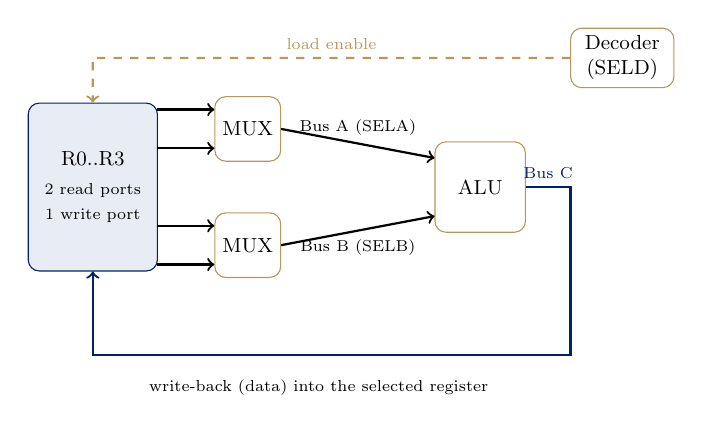
\begin{tikzpicture}[scale=0.82, transform shape,
      every node/.style={font=\small}]
    \node[draw=primary-blue, fill=light-bg, rounded corners,
          minimum width=2.0cm, minimum height=2.6cm, align=center] (RF) at (0,0) {R0..R3\\[2pt]\scriptsize 2 read ports\\\scriptsize 1 write port};
    \node[draw=primary-gold, fill=white, rounded corners,
          minimum width=1.0cm, minimum height=1.0cm, align=center] (MUXA) at (2.4,0.9) {MUX};
    \node[draw=primary-gold, fill=white, rounded corners,
          minimum width=1.0cm, minimum height=1.0cm, align=center] (MUXB) at (2.4,-0.9) {MUX};
    \draw[->, thick] (1.0,1.2) -- (MUXA.west |- 0,1.2);
    \draw[->, thick] (1.0,0.6) -- (MUXA.west |- 0,0.6);
    \draw[->, thick] (1.0,-0.6) -- (MUXB.west |- 0,-0.6);
    \draw[->, thick] (1.0,-1.2) -- (MUXB.west |- 0,-1.2);
    \node[draw=primary-gold, fill=white, rounded corners,
          minimum width=1.4cm, minimum height=1.4cm, align=center] (ALU) at (6.0,0) {ALU};
    \draw[->, thick] (MUXA.east) -- node[midway, above, font=\scriptsize] {Bus A (SELA)} (ALU.west |- 0,0.45);
    \draw[->, thick] (MUXB.east) -- node[midway, below, font=\scriptsize] {Bus B (SELB)} (ALU.west |- 0,-0.45);
    \draw[->, thick, primary-blue] (ALU.east) -- node[midway, above, font=\scriptsize] {Bus C}
          (7.4,0) -- (7.4,-2.6) -- (0,-2.6) -- (RF.south);
    \node[font=\scriptsize] at (3.5,-3.1) {write-back (data) into the selected register};
    \node[draw=primary-gold, fill=white, rounded corners,
          minimum width=1.6cm, minimum height=0.9cm, align=center] (DEC) at (8.2,2.0) {Decoder\\(SELD)};
    \draw[->, thick, primary-gold, dashed] (DEC.west) -- node[midway, above, font=\scriptsize] {load enable} (0,2.0) -- (RF.north);
  \end{tikzpicture}
  \caption{The three-bus CPU datapath --- cf.\ Mano, \textit{Computer System Architecture}, 3rd ed., Fig.~8-2, p.243 (``Registers with common ALU''); the same three-bus principle is also presented in Hamacher, \textit{Computer Organization}, Ch.~7 \cite{Mano1993_computer_system_architecture,Hamacher2002_computer_organization}.}
  \label{fig:three-bus}
\end{figure}

\begin{example}[\texttt{R1} $\gets$ \texttt{R2 + R3} on Three Buses]
\begin{center}
\small
\begin{tabular}{@{}cp{3.6cm}p{3.0cm}p{4.6cm}@{}}
\toprule
\textbf{Step} & \textbf{RTL} & \textbf{On the buses} & \textbf{What happens} \\
\midrule
$T_1$ & $R1 \gets [R2] + [R3]$ & $A = [R2]$, $B = [R3]$, $C = $result & Both operands read \emph{and} the ALU output written back, all in one cycle \\
\bottomrule
\end{tabular}
\end{center}
This is \textbf{1 control step} for the identical \texttt{ADD} that took 3 steps on the single-bus organization --- the same instruction, the same ALU, but different wiring. The ALU no longer needs a \texttt{Y} buffer at all, because both of its inputs arrive in the same cycle directly from the register file, and Bus C lets the result be written back in that same cycle precisely because it is not competing with Bus A or Bus B for the same wire. The sequential bottleneck that forced the single-bus design into three steps simply does not exist here.
\end{example}

\subsection{Trade-offs}

Most two-operand register instructions now complete their data movement in a single control step, and no \texttt{Y}/\texttt{Z} buffering is needed for the common case. The cost is three times the bus wiring, plus the multiplexers needed to route any register onto any of the three buses, and control logic that must correctly drive three buses every cycle rather than one.

\subsection{Single-Bus versus Three-Bus: A Comparison}

\begin{center}
\small
\begin{tabular}{@{}p{3.0cm}p{4.2cm}p{4.2cm}@{}}
\toprule
 & \textbf{Single bus} & \textbf{Three bus} \\
\midrule
Wiring cost & Low (one bus) & High (three buses + muxes) \\
Cycles for $R1 \gets R2{+}R3$ & 3 ($T_1, T_2, T_3$) & 1 ($T_1$) \\
Extra registers needed & Y, Z (buffering) & None (common case) \\
Control logic & Simple, uniform & More complex, more signals \\
Best fit & Cost-sensitive designs & Performance-sensitive designs \\
\bottomrule
\end{tabular}
\end{center}

Neither design is ``correct'' in an absolute sense --- they sit at different points on the same cost/speed trade-off curve.

\subsection{Design-Space Limits: Why Not Ten Buses?}

If three buses beat one, why not build a CPU with ten, or a hundred? Every additional bus needs its own wiring and its own multiplexer logic at every register, so cost grows with the number of buses rather than being free. Beyond that, most instructions need only two operand reads and one result write, so past three buses there is little left to parallelize \emph{within a single instruction}. Real speedups beyond this point come from a different idea entirely: overlapping \emph{different} instructions in time, which is exactly what pipelining (Week 11) does.

\section{Synthesis and Summary}

\subsection{Interaction Between Addressing Mode and Bus Organization}

Addressing modes carry a bus-organization cost of their own. Recall indirect addressing's two memory reads to resolve $\text{EA}$: on a single-bus CPU, each of those reads is itself another multi-step bus transaction, so the ``expensive'' addressing mode and the ``expensive'' bus organization compound rather than simply adding. Cheap addressing (immediate, register) paired with a cheap bus (single) yields minimal hardware but more cycles per instruction; expensive addressing (indirect) paired with an expensive bus (three-bus) can still be fast, but every design choice is paid for somewhere, in wires or in cycles, never for free.

\subsection{Summary}

An \textbf{addressing mode} is the rule for computing $\text{EA}$ from an instruction's address field; each mode trades flexibility against extra memory or bus reads (Section~\ref{sec:addressing-modes}). \textbf{RTL notation} ($R \gets [\cdot]$, $M[\text{EA}]$, control steps $T_1, T_2, \dots$) is how hardware-level data movement is described precisely. A \textbf{single-bus organization} is cheap to wire, moves data sequentially, needs \texttt{Y}/\texttt{Z} buffering, and costs more cycles per instruction. A \textbf{multiple-bus organization} allows parallel register reads and writes, costs fewer cycles per instruction, but needs more wiring and more complex control. The same instruction, on the same ALU, with different wiring, takes 3 cycles versus 1 --- the cost/speed trade-off, made concrete. This chapter built seven addressing modes and two competing bus organizations, but in every worked trace $T_1, T_2, T_3$ were written by hand; Chapter 6 builds the control unit that generates that sequence automatically, for every instruction, every time it runs.

\bibliographystyle{plain}
\bibliography{../../Bibliography_base}

\end{document}
